\chapter{Nanopype Processing Pipeline}
\label{sec:nanopype}

Long-read third-generation nanopore sequencing enables researchers to now address a range of questions that are difficult to tackle with short read approaches. The rapidly expanding user base and continuously increasing throughput have sparked the development of a growing number of specialized analysis tools. However, streamlined processing of nanopore datasets using reproducible and transparent workflows is still lacking. Here we present Nanopype, a nanopore data processing pipeline that integrates a diverse set of established bioinformatics software while maintaining consistent and standardized output formats. Seamless integration into compute cluster environments makes the framework suitable for high-throughput applications. As a result, Nanopype facilitates comparability of nanopore data analysis workflows and thereby should enhance the reproducibility of biological insights. Nanopype is available at \textit{https://github.com/giesselmann/nanopype}.

\begin{figure}[h]
    \centering
    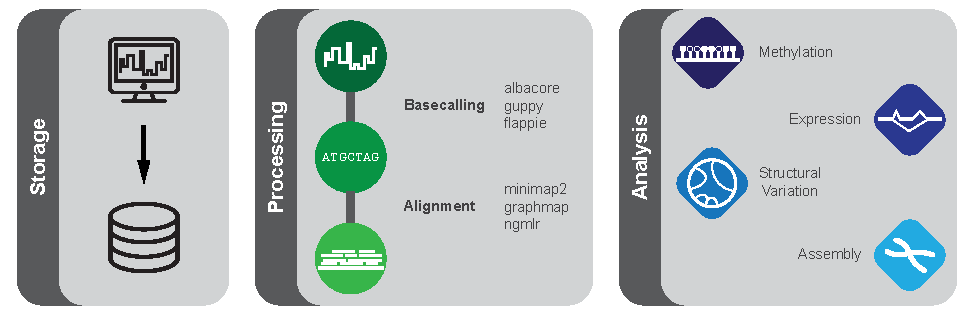
\includegraphics[width=1.0\textwidth]{figures/nanopype/GA.pdf}
    \label{fig:nanopype:ga}
\end{figure}

\textbf{Note:} This chapter is based on the publication P. Giesselmann et al. \textit{Nanopype: a modular and scalable nanopore data processing pipeline}, Bioinformatics, 2019 and contains text from the original paper.

The chapter starts with a brief \textbf{background} in \ref{sec:nanopype:background} followed by high-level pipeline \textbf{design} decisions covering storage, tool encapsulation and reproducibility in section \ref{sec:nanopype:design}.
The \textbf{installation} section \ref{sec:nanopype:installation} illustrates the setup and configuration of the pipeline in different environments. Grouped into \textbf{modules} individual tools are highlighted in section \ref{sec:nanopype:modules}.
Finally the \textbf{usage} on a daily production level is outlined in section \ref{sec:nanopype:usage}.




\section{Background}
\label{sec:nanopype:background}
Third-generation sequencing techniques are currently introducing new perspectives to the field of genome analysis by generating previously unattainable read lengths with averages in the tens of thousands of nucleotides. Among other devices distributed by Oxford Nanopore Technologies (ONT), the MinION in particular is gaining prominence. In brief, the nanopore sequencing process is based on guiding a nucleotide polymer through a pore inserted in a membrane while measuring a change in ionic current as a proxy signal over time. This signal is then interpreted to determine the underlying DNA or RNA sequence. The nanopore technology enables direct readout of sequences from individual DNA or RNA molecules including base modifications since no synthesis or amplification is required.

Due to constant development and improvement of applications, frequent reprocessing of the raw signal and downstream data is necessary. Thus, novel archiving and processing strategies are needed for data storage and handling that scale with the large amount of data produced by the MinION sequencer. This will be even more relevant as higher throughput devices such as the PromethION become more widely available. Furthermore, a limiting factor of the applicability of this new technology are the currently available, research-grade software packages for nanopore long-read data analyses. These tend to be difficult to install and require complex software environments. Despite the growing number of recently developed algorithms \cite{Magi2018}, primary data processing remains challenging due to stand alone tools without congruent data formats and requirements. 
Current examples of nanopore data processing pipelines are Katuali\footnote{github.com/nanoporetech/katuali} for basecalling and assembly and Pinfish\footnote{github.com/nanoporetech/pipeline-pinfish-analysis} for RNA isoform detection from cDNA and direct RNA sequencing experiments. However they have been developed to perform specific analysis workflows without integrated handling of the critical raw data storage or version control of wrapped tools.

To overcome these issues, we have developed Nanopype, a pipeline designed explicitly for streamlined and automated nanopore long read processing. Apart from the integration of essential base calling, quality control, and alignment tools, we facilitate a set of published analysis applications for barcode demultiplexing, DNA methylation readout, structural variant calling, RNA isoform detection and genome assembly. 
Based on the Snakemake engine \cite{Koester2012} our method integrates established error handling and uniform output structures across multiple experiments. Furthermore, Nanopype can be run in a parallel setup on both, single computers and server clusters. Deployed as a python module, Nanopype is mostly build from source with encapsulated routines to simplify the initial setup and integration into existing environments. Additionally, we provide Singularity images for all modules and an automatically built all-in-one Docker container. This enables the usage of the pipeline for both, less bioinformatically experienced experimental scientists and bioinformaticians. Lastly, Nanopype provides a well-defined framework for standardized processing independent of the underlying operating system.




\section{Design}
\label{sec:nanopype:design}
Nanopype’s core element is a modular setup to easily update existing tools and to seamlessly integrate the latest developments. Nonetheless, each pipeline release is freezing the included tool versions to guarantee reproducible results. In a nutshell, Nanopype has been designed around three key components: raw data storage, tool encapsulation and standardized directory structures that mirror the applied toolchain.

\subsection{Storage}
\label{subsec:nanopype:storage}
The first core design component is the consistent storage of the raw signal data from any ONT sequencer. 
Raw nanopore reads are stored in FAST5 files, an ONT specification of the universal HDF5 file format. Initially the sequencers exported one file per read, resulting in hundreds of thousands of files per sequencing run. 
The number of files generated could, especially on Linux file systems, disrupt background services such as nightly mirrors and backups.
Nanopype is backward compatible with datasets of single read FAST5 files, for which we provide a module to import and package single reads into TAR archive batches.

More recently ONT utilized the full functionality of the HDF5 format with groups (comparable to directories), datasets (structured arrays of primitive data types) and attributes (single values for meta information) and released the multi-read-FAST5 format. The new format typically groups 4000 reads into a single file, resulting in notable improvements regarding copy and synchronization tasks.

In combination with the Nanopype pipeline we propose a multi-device and multi-user nanopore sequencing setup (Fig. \ref{fig:nanopype:storage}). Provided with a suitable server infrastructure the design supports processing of multiple sequencing runs per week from both local and remotely connected devices. Deploying \textit{syncthing}\footnote{https://github.com/syncthing/syncthing} on device and server side, we synchronize the output folder from the \textit{MinKNOW} sequencing software with device specific folders in a central spooling area.
After completion of the sequencing, the data is moved to the active storage, the file ownership is changed to a particular \textit{data user} and files are made write protected (Fig. \ref{fig:nanopype:storage}).

\begin{figure}[h]
	\centering
	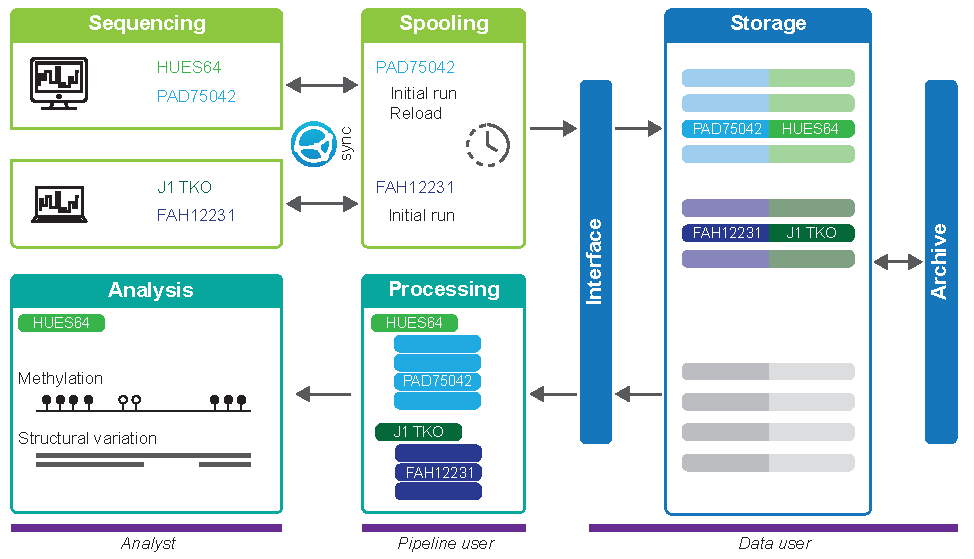
\includegraphics[width=1.0\textwidth]{figures/nanopype/storage.pdf}
	\captionsetup{format=plain}
	\caption[Nanopype data flow]{Data flow for multi-sequencer and multi-user setup: Raw data generated on local or remote devices is synchronized into local spooling directory. Complete runs with meta information are stored with read-only access and archived on tape. Processing combines multiple sequencing runs of the same sample and provides basic readout for downstream analysis.}
	\label{fig:nanopype:storage}
\end{figure}

The active storage contains one folder per sequencing run following a uniform naming pattern of date, flow cell ID, flow cell type, sequencing kit and a sequence of arbitrary user tags e.g.:

\begin{center}
	20200401\_FAH12345\_FLO-MIN106\_SQK-LSK109\_HUES64\_WT
\end{center}

From the active storage, sequencing runs can be archived on e.g. tape drives for long term data retention. For the processing, sequencing runs are mapped into an interface (a directory with softlinks into the active storage). This additional layer allows the distribution of raw data across multiple physical devices, while maintaining consistent access.
The raw data archive forms the basis for any downstream analyses and enables smooth re-processing of legacy datasets as soon as for example improved basecalling algorithms become available.

\subsection{Encapsulation}
\label{subsec:nanopype:encapsulation}
The installation of experimental software packages still being actively developed with complex library dependencies can be time-consuming, but remains essential to make use of the current-generation nanopore analysis workflows. On a base level, Nanopype uses Snakemake rules to wrap the build from source and installation process of its dependencies and therefore does not require root privileges for the setup on common Linux and MacOS systems. The build from source is the most customizable setup option and moreover allows the integration into complex, preexisting environments.

The internal wrappers are used to automatically build and deploy Singularity images for preset modules and pipeline versions. The images are automatically pulled once a module is used. This mechanism enables the complete function set of Snakemake and Nanopype while only requiring a system-wide Python and Singularity installation. In contrast to Docker, the execution of Singularity containers does not require root privileges on the target system.
An all-in-one Singularity container is provided, wrapping the entire pipeline into a single environment. Primarily aimed for stand-alone usage, Windows systems, and for initial testing, this method does not offer support for cluster computation. 

While greatly simplifying the installation process, containerized software comes at the cost of the container size. Whereas the \textit{minimap2} binary alone is 1 MB small, the size of the Nanopype alignment image is 314 MB due to integration of alignment tools, samtools, libraries and the Ubuntu kernel. Especially within distributed environments this means, that each cluster job needs to fetch these images from a file server, leading to noticeable overhead depending on the jobs core function. 


\subsection{Transparency}
\label{subsec:nanopype:transparency}
Nanopype follows the Snakemake concept of output file driven computation: a single user command typically provokes transparent processing of any required intermediate result. Preexisting tools are integrated into consistent workflows and provide standard output formats to connect to workflows of established next-generation sequencing data analysis tools. The processing and subsequent output is intuitively organized in modules and underlying application directories (Fig. \ref{fig:nanopype:dir_tree}).

\begin{figure}[h]
	\centering
	\begin{minipage}{.7\linewidth}
	\dirtree{%
		.1 ./.
		.2 sequences/.
		.3 guppy/.
		.4 batches/.
		.4 Hues8.fast.fastq.gz.
		.2 alignments/.
		.3 ngmlr/.
		.4 guppy/.
		.5 batches/.
		.5 Hues8.fast.hg38.bam.
		.2 methylation/.
		.3 nanopolish/.
		.4 ngmlr/.
		.5 guppy/.
		.6 batches/.
		.6 Hues8.fast.10x.hg38.bw.
	}
	\end{minipage}
	\captionsetup{format=plain}
	\caption[Possible nanopype output directory]{Possible nanopype output directory structure after basecalling, alignment and methylation detection. Top level directories represent pipeline modules with the applied tools in subjacent levels. \textbf{Hues8.fast} is the user defined tag of the output, in this case for the hESC HUES8 and guppy basecalling in fast mode. \textbf{10x} is the coverage wildcard indicating to filter for CpGs with at least 10 reads coverage. \textbf{Hg38} defines the reference genome and \textbf{.bw} the output file format.}
	\label{fig:nanopype:dir_tree}
\end{figure}




\section{Installation}
\label{sec:nanopype:installation}

Consistent versioning of source and container builds ensures reproducibility independent of the installation method.

\subsection{Source}



%\begin{itemize}
%	\item dependencies
%	\item build rules
%	\item tests
%\end{itemize}

\subsection{Container}

Docker and Singularity enable the encapsulation of tools and dependencies into virtualized software containers. Packaging libraries and data, these containers can be executed on any operating system with just the virtualization set up. Due to the free availability, Nanopype module images are build as Docker containers on \textit{https://hub.docker.com/u/nanopype/}, but executed by Singularity from the Snakemake backend. Webhooks from Github trigger builds on each push to master and development branch. Tagged commits (e.g. \textit{v0.10.0}) to the master branch are build as tagged images. Upon execution the pipeline version is inferred from the git tag and associated Docker images are pulled as needed for the workflow.


In order to minimize the size of each container, most Nanopype modules rely on a staged build process. Within the Dockerfile two separate images are configured. The first build stage contains installations of toolchains and development libraries. Bioinformatic tools required by Nanopype are compiled and linked in this stage. The build process for the alignment module is partially shown in listing \ref{lst:nanopype:docker}.

\lstinputlisting[language=docker, caption=Staged Docker build, label=lst:nanopype:docker]{listings/nanopype/docker_staged.txt}

A subsequent runtime stage copies the binaries from the build stage and requires only the installation of libraries for dynamically linked executables. The build stage is dropped in the final compressed image.


\subsection{Configuration}

Nanopype has two configuration layers: The central environment configuration \textit{env.yaml} covers application paths and reference genomes and is set up independent of installation method and operating system once. The environment configuration is stored in the installation directory. If a compute cluster is available the respective Snakemake configuration is only needed once per Nanopype installation and explained here by the example of a custom scheduler called mxq.

For each project an additional workflow configuration is required providing data sources, tool flags and parameters. The workflow config file \textit{nanopype.yaml} is expected in the root of each project directory. Configuration files are in .yaml format.


%\begin{itemize}
%	\item environment
%	\item workflow
%	\item profiles
%	\item cluster
%	\subitem shadow prefix
%	\item GPU support
%\end{itemize}




\section{Modules}
\label{sec:nanopype:modules}
Nanopype’s backbone consists of a set of modules that resolve a specific task, like basecalling, alignment or further downstream analyses. If available, alternative applications are provided for the same task and grouped into a module with a coherent output format. Integrating first and foremost low-level nanopore data processing applications provided by ONT, established community developed software packages have been included in the first Nanopype release, as well.


\subsection{Basecalling}
\label{subsec:nanopype:basecalling}
The basecalling module translates raw nanopore signals into nucleotide sequences and is utilized by most subsequent pipeline layers. With the initial release, we include the established packages Guppy, Albacore, and Flappie, all provided by ONT \cite{Wick2019}. The default basecaller package is set to the recently released Guppy. Albacore is supported for backward compatibility but deprecated by ONT. The experimental Flappie is ONT’s first DNA methylation-aware basecaller. It extends the usual four-letter nucleotide alphabet by a fifth letter for methylated cytosine in CpG contexts. For all basecallers, the output is the standardized FASTQ and supplemented by us with a basic quality control summary.


\subsection{Alignment}
\label{subsec:nanopype:alignment}
The core functionality of the pipeline is the alignment of reads against a reference genome or draft assembly. Here, we provide three different aligners with distinct advantages, which make them favorable for different applications downstream. While Minimap2 \cite{Li2018} is a fast, low memory footprint solution suitable for both DNA and RNA alignments, GraphMap \cite{Sovic2016} is a sensitive aligner but with comparably high memory requirements. NGMLR \cite{Sedlazeck2018} is the recommended tool for the structural variation module. Any combination of basecalling, alignment, and reference genome is supported and reports BAM format files.


\subsection{DNA methylation}
\label{subsec:nanopype:methylation}
Sequencing without prior DNA amplification enables the direct readout of DNA base modifications. The current state of the art approach, Nanopolish \cite{Simpson2017} as well as the more experimental flip-flop basecaller Flappie, are incorporated into Nanopype. Subsequently, Nanopype splits Flappie’s atypical sequence output into standard FASTQ and methylation status. DNA methylation at CpG dinucleotides of both tools is reported in a table format for single reads. Furthermore, we provide common bedGraph and bigWig files for genome-wide methylation tracks and thus enable downstream processing using established workflows, e.g., calling of differential methylated regions and comparison to bisulfite sequencing.

\begin{figure}[h]
	\centering
	\includegraphics[width=1.0\textwidth]{figures/nanopype/sr_methylation.pdf}
	\captionsetup{format=plain}
	\caption[Nanopype single read methylation track]{Nanopype single read methylation track of nanopore sequenced HUES8 hESCs. Mean methylation track of CpGs with >=10\textit{x} coverage. Single read methylation computed from original alignment by substituting unmethylated Cs to Ts (imitated bisulfite conversion, blue). Unclassified sites (abs. nanopolish log-likelihood-ratio < 2.5) are substituted with As and appear as mismatches (orange). All remaining mismatches in the nanopore reads are replaced with the genomic sequence. Shown are reads overlapping DIRAS3 as imprinted gene on genome build hg38, grouped by allele and shaded by strand.}
	\label{fig:nanopype:sr_methylation}
\end{figure}


\subsection{Structural variation}
\label{subsec:nanopype:sv}
Detection and characterization of structural variation play a central role in cancer research and population genetics. Long read sequencing particularly facilitates investigation of variants with unprecedented accuracy and resolution. Therefore, Nanopype encompasses the variant caller Sniffles \cite{Sedlazeck2018} and provides output in the standard variant calling format (VCF).


\subsection{Transcriptome}
\label{subsec:nanopype:transcriptom}
Another application of the long-read nanopore technology is sequencing of cDNA and RNA molecules directly. Recovery of full-length transcripts enables, for instance, the detection of alternatively spliced isoforms and is implemented in Nanopype using the Pinfish package. The output of polished transcripts is provided in the GFF format.

\begin{figure}[h]
	\centering
	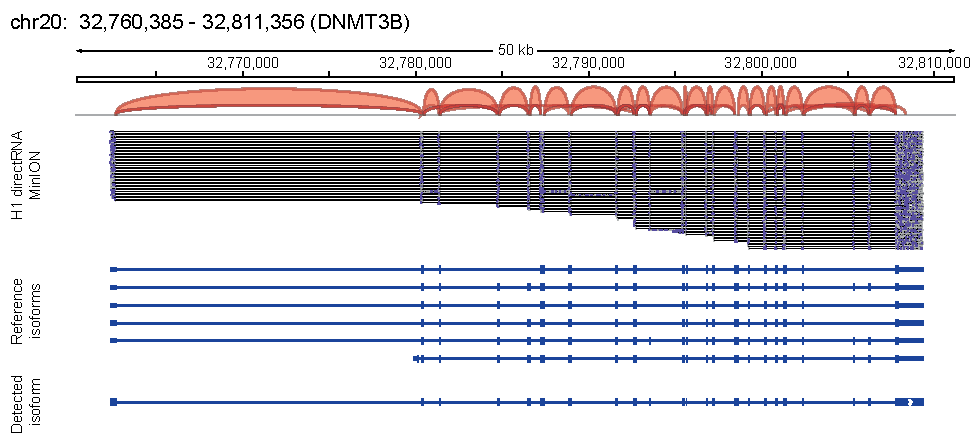
\includegraphics[width=1.0\textwidth]{figures/nanopype/rna_isoforms.pdf}
	\captionsetup{format=plain}
	\caption[Nanopore direct RNA sequencing]{Nanopore direct RNA sequencing of hESC H1 from one MinION flow cell. Shown are \textit{minimap2} splice-aligned reads spanning DNMT3B, obtained by using the RNA sequencing without amplification. The isoform detected from the \textit{Pinfish} package matches one of the reference isoforms.}
	\label{fig:nanopype:rna_isoforms}
\end{figure}


\subsection{Genome Assembly}
\label{subsec:nanopype:assembly}



Complemented by samtools \cite{Li2009}, bedtools \cite{Quinlan2010} and UCSCtools \cite{Kent2010} our pipeline establishes a comprehensive framework for ONT sequencing data processing.




\section{Usage}
\label{sec:nanopype:usage}
Due to the functional range of Nanopype, dependent on the operating system, and selected installation method the setup can require advanced information technology knowledge. However, after deployment, the subsequent usage is straightforward given basic command line understanding. Complete Nanopype workflows can be executed with a single concise command line call. For instance, local processing of multiple flow cells into a collective genome-wide methylation track of at least 5x coverage on reference hg38 requires only the following line:

\begin{lstlisting}[language=sh, caption=Snakemake example]
snakemake --snakefile ~/nanopype/Snakefile methylation/nanopolish/ngmlr/guppy/Hues8.5x.hg38.bw
\end{lstlisting}

This command invokes basecalling, alignment and methylation detection using declared tools without further user interaction. The basecalling and alignment outputs are kept and can be reused to avoid redundant processing.

%\begin{itemize}
%	\item tag concept
%	\item special tag introduction
%\end{itemize}


\subsection{Batch processing}
The automatic distribution of workflows into independent batches enables efficient handling of high-throughput experiments. This feature becomes particularly relevant for scaling in cluster environments and most importantly in case of terminated or failed batches. As a result, only failed batches require reprocessing by resuming the workflow from where it left off, using the same command which enhances the overall error robustness.
The source and Singularity versions of Nanopype do not interfere with the extensive cluster support of Snakemake.

%\begin{itemize}
%	\item raw signal batches
%	\item temporary data
%	\item sorting
%	\item command line length, open files
%	\item non batch modules e.g. sv
%\end{itemize}


\subsection{Barcoding}
Demultiplexing: Barcoded sequencing allows pooling of multiple samples on a single flow-cell. The demultiplexing module uses Deepbinner \cite{Wick2018} to assign a barcode label to the individual reads. Thus, sequencing of comparable small bacterial genomes can be efficiently parallelized to use the available sequencing depth optimally.

Indexing the content of both, packaged and multi-FAST5 output enables the fast retrieval of individual reads. 


\subsection{Logging and Reports}

%\begin{itemize}
%	\item cluster job logging
%	\item log of config values into tagged logfile
%\end{itemize}




\section{Summary}
\label{sec:nanopype:summary}
Here we present Nanopype, a modular and easy-to-use data processing pipeline with a detailed online documentation, specifically designed to handle nanopore sequenced long-read data.
Nanopype provides end-to-end processing of the raw sequencer signal into standard data formats and consequently closes the gap to downstream next-generation sequencing algorithms. Single command invocations of entire workflows reduce the hands-on-time for users to receive the desired output. Implicitly, this also lowers the potential of user mistakes and deviations in processing of multiple data sets. As a consequence, workflows are easier to reproduce with fixed versions among datasets or repeated with improved tool releases on existing ones.
Nanopype is implemented as a python package and additionally provides pre-built and versioned Singluarity and Docker images, making it favorable for effective usage in cluster and single computer environments. The pipeline design ensures portability and version controlled usage of the implemented tools, to enable consistent results across platforms.


